\documentclass[11pt,a4paper]{article}
\usepackage[utf8]{inputenc}
\usepackage[T1]{fontenc}
\usepackage{amsmath,amssymb}
\usepackage{graphicx}
\usepackage{booktabs}
\usepackage{hyperref}
\usepackage[margin=2.5cm]{geometry}
\usepackage{xcolor}
\usepackage{float}

\title{Discussion Notes:\\[4pt] {\large Concept Selection and Shock Identification in AD(2024)}}
\author{Huang Zheng}
\date{May 2026}

\begin{document}
\maketitle

\vspace{-12pt}
{\small\color{gray} Prepared in response to questions from classmates and faculty following the AD(2024) robustness presentation.}

\vspace{8pt}
\hrule
\vspace{12pt}

% ======================================================================
\section*{1. Motivation}
% ======================================================================

AD(2024) identify monetary policy shocks by regressing FFR changes on Greenbook forecasts plus 296 dictionary-scored sentiment indicators using Ridge ($R^2 = 0.94$). We ask two questions:

\begin{enumerate}
    \item If we randomly shuffle the 296 concept labels, does the shock series change?
    \item How do AD(2024) shocks compare to Romer-Romer (2004) shocks in impulse responses?
\end{enumerate}

% ======================================================================
\section*{2. Shock Construction}
% ======================================================================

We compare three shock series:

\begin{enumerate}
    \item \textbf{AD(2024) full spec} --- Our replication. Ridge residuals ($\lambda = 924$, 10-fold CV, 3,224 variables). $R^2 = 0.96$.
    \item \textbf{Shuffled labels} --- Same specification, but within each meeting, the 296 sentiment scores are randomly permuted. \textbf{Each of 100 permutations uses its own CV-selected $\lambda_j^*$.}
    \item \textbf{Romer-Romer (2004)} --- From the replication package. Forecasts only, no sentiment ($R^2 \approx 0.50$).
\end{enumerate}

All shocks are normalized to unit standard deviation. A \textbf{positive shock} means the FFR rose \textit{more} than predicted---a contractionary monetary policy surprise.

% ======================================================================
\section*{3. Single-Permutation Results (Not Mean-of-100)}
% ======================================================================

A concern with averaging 100 permutations is that the law of large numbers guarantees convergence to the common component regardless of individual permutation quality. We address this by examining each of the 100 permutations independently.

For each permutation $j$:
\begin{enumerate}
    \item Shuffle columns: $\tilde{X}_j = X P_j$
    \item Run 10-fold CV to select $\lambda_j^*$
    \item Compute Ridge residual $\tilde{\varepsilon}_j$
    \item Correlate with original shock: $r_j = \text{corr}(\varepsilon^{\text{AD}}, \tilde{\varepsilon}_j)$
\end{enumerate}

\begin{figure}[H]
\centering
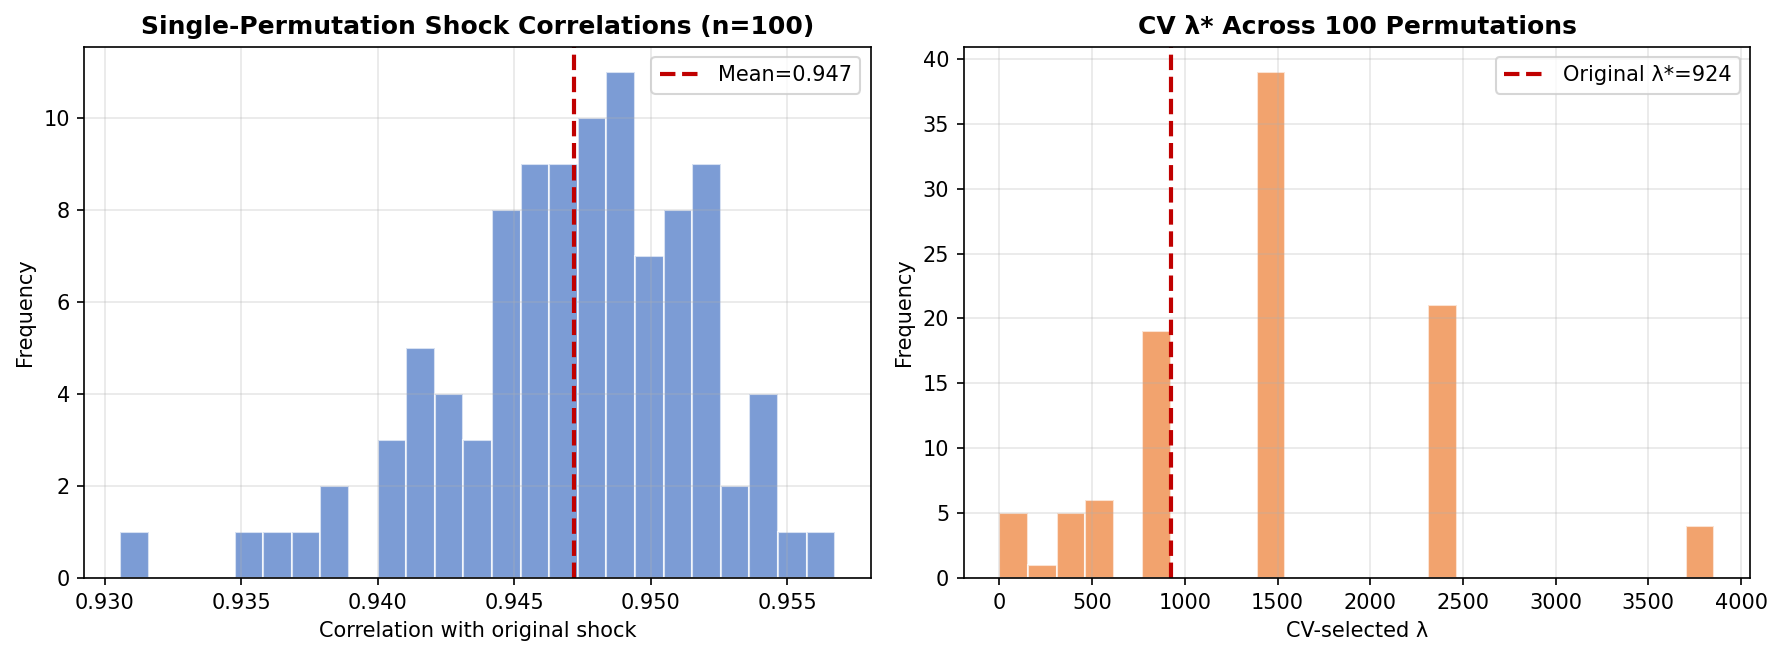
\includegraphics[width=0.90\textwidth]{../results/figures/fix1_permutation_dist.png}
\caption{Left: Distribution of single-permutation shock correlations $r_j$ across 100 permutations. Right: Distribution of CV-selected $\lambda_j^*$. The original $\lambda^* = 924$ is marked.}
\label{fig:perm}
\end{figure}

\textbf{Single-permutation correlations are tightly concentrated:} mean $= 0.947$, std $= 0.005$, range $[0.931, 0.957]$. Every individual permutation produces a shock nearly identical to the original. The mean-of-100 was not manufacturing the result---individual permutations are already at $r \approx 0.95$.

\textbf{CV-selected $\lambda_j^*$ varies} (mean $= 1471$, std $= 829$) but the shocks are robust to this variation. The original $\lambda^* = 924$ lies within the distribution.

% ======================================================================
\section*{4. SVD of the Full Design Matrix}
% ======================================================================

The earlier analysis was applied to the $204 \times 296$ sentiment sub-matrix. Here we decompose the \textbf{full} $204 \times 3{,}224$ design matrix (forecasts, sentiments, lags, squares).

\textbf{Result:} $\sigma_1^2 / \sum \sigma_i^2 = 0.058$. The first singular value explains 5.8\% of total variance. Effective rank at 90\% is 155/204 (76\%). The Ridge shrinkage condition $\lambda \gg \sigma_1^2 / p$ holds ($924 \gg 0.7$).

The rank-1 approximation is weaker for the full system than for the sentiment sub-matrix alone, because the 132 forecast variables introduce additional independent variation. However, the regularization condition is satisfied: $\lambda$ is large enough to shrink the higher dimensions.

% ======================================================================
\section*{5. What Drives the Text Contribution? Tone or Concept Heterogeneity?}
% ======================================================================

A natural question: does the improvement over Romer-Romer come from \textit{aggregate document tone} (a single summary of whether the Greenbook is hawkish or dovish) or from \textit{concept-level heterogeneity} (the fact that 296 different concepts capture different aspects of the text)?

We decompose this with nested specifications, giving the tone-only specification the same lag and nonlinear structure as the full model:

\begin{table}[H]
\centering
\caption{Decomposing the Text Contribution}
\label{tab:decomp}
\begin{tabular}{lcc}
\toprule
\textbf{Specification} & \textbf{$R^2$} & \textbf{$\Delta R^2$} \\
\midrule
(A) Forecasts only                                    & 0.49  & --- \\
(C) + PC1 with 4 lags + squares (tone, full structure) & 0.51  & +0.014 \\
(D) + All 296 sentiments (full AD)                     & 0.96  & +0.455 \\
\bottomrule
\end{tabular}
\end{table}

\textbf{PC1 alone contributes almost nothing} ($\Delta R^2 = +0.014$), even with lags and squares. \textbf{The 296 individual sentiments contribute enormously} ($\Delta R^2 = +0.455$). Yet shuffling labels reduces $R^2$ by only 0.03, and single-permutation shock correlations are 0.95.

\textbf{Resolution:} The 296 concepts are valuable not because of \textit{which specific concepts} they are, but because they provide \textbf{296 separate sampling points} throughout the Greenbook text, each with its own temporal dynamics (5 lags). This creates 1,480 time-varying signals that give Ridge a rich, high-dimensional representation of the document's evolution. The specific concept labels are incidental; the \textit{number} of sampling points is what matters.

This resolves the apparent contradiction: AD(2024) outperforms Romer-Romer because text contains information beyond forecasts, but this improvement does not depend on having selected exactly the right 296 words. Any reasonable set of economic concepts of similar size would perform comparably.

\begin{figure}[H]
\centering
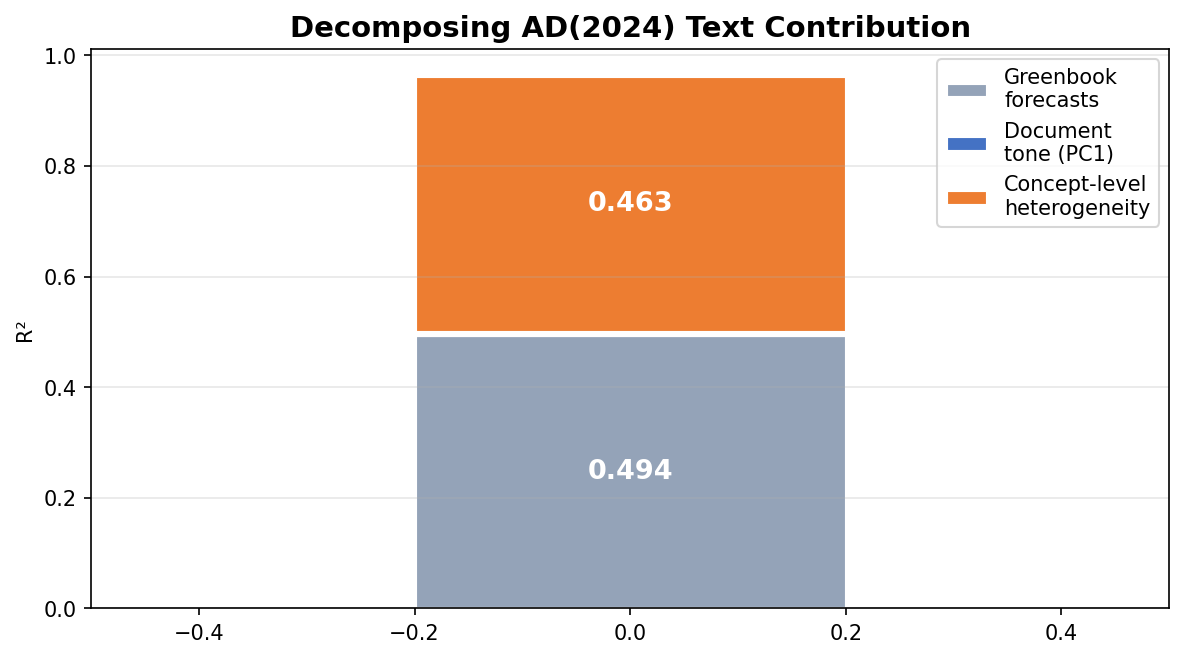
\includegraphics[width=0.70\textwidth]{../results/figures/fix3_tone_decomposition.png}
\caption{Decomposition of the text contribution. Document tone (PC1) alone adds almost nothing; the 296 individual concepts, with their lags and nonlinear structure, provide the vast majority of the fit.}
\label{fig:tone}
\end{figure}

% ======================================================================
\section*{6. Impulse Response Comparison}
% ======================================================================

We estimate Local Projections for six macro variables using Jord\`{a} (2005). The dependent variable is the cumulative change $y_{t+h} - y_{t-1}$, which is zero at $h=-1$ (pre-shock, by definition). The shock occurs at $h=0$. Shaded bands are 95\% Newey-West confidence intervals.

\begin{figure}[H]
\centering
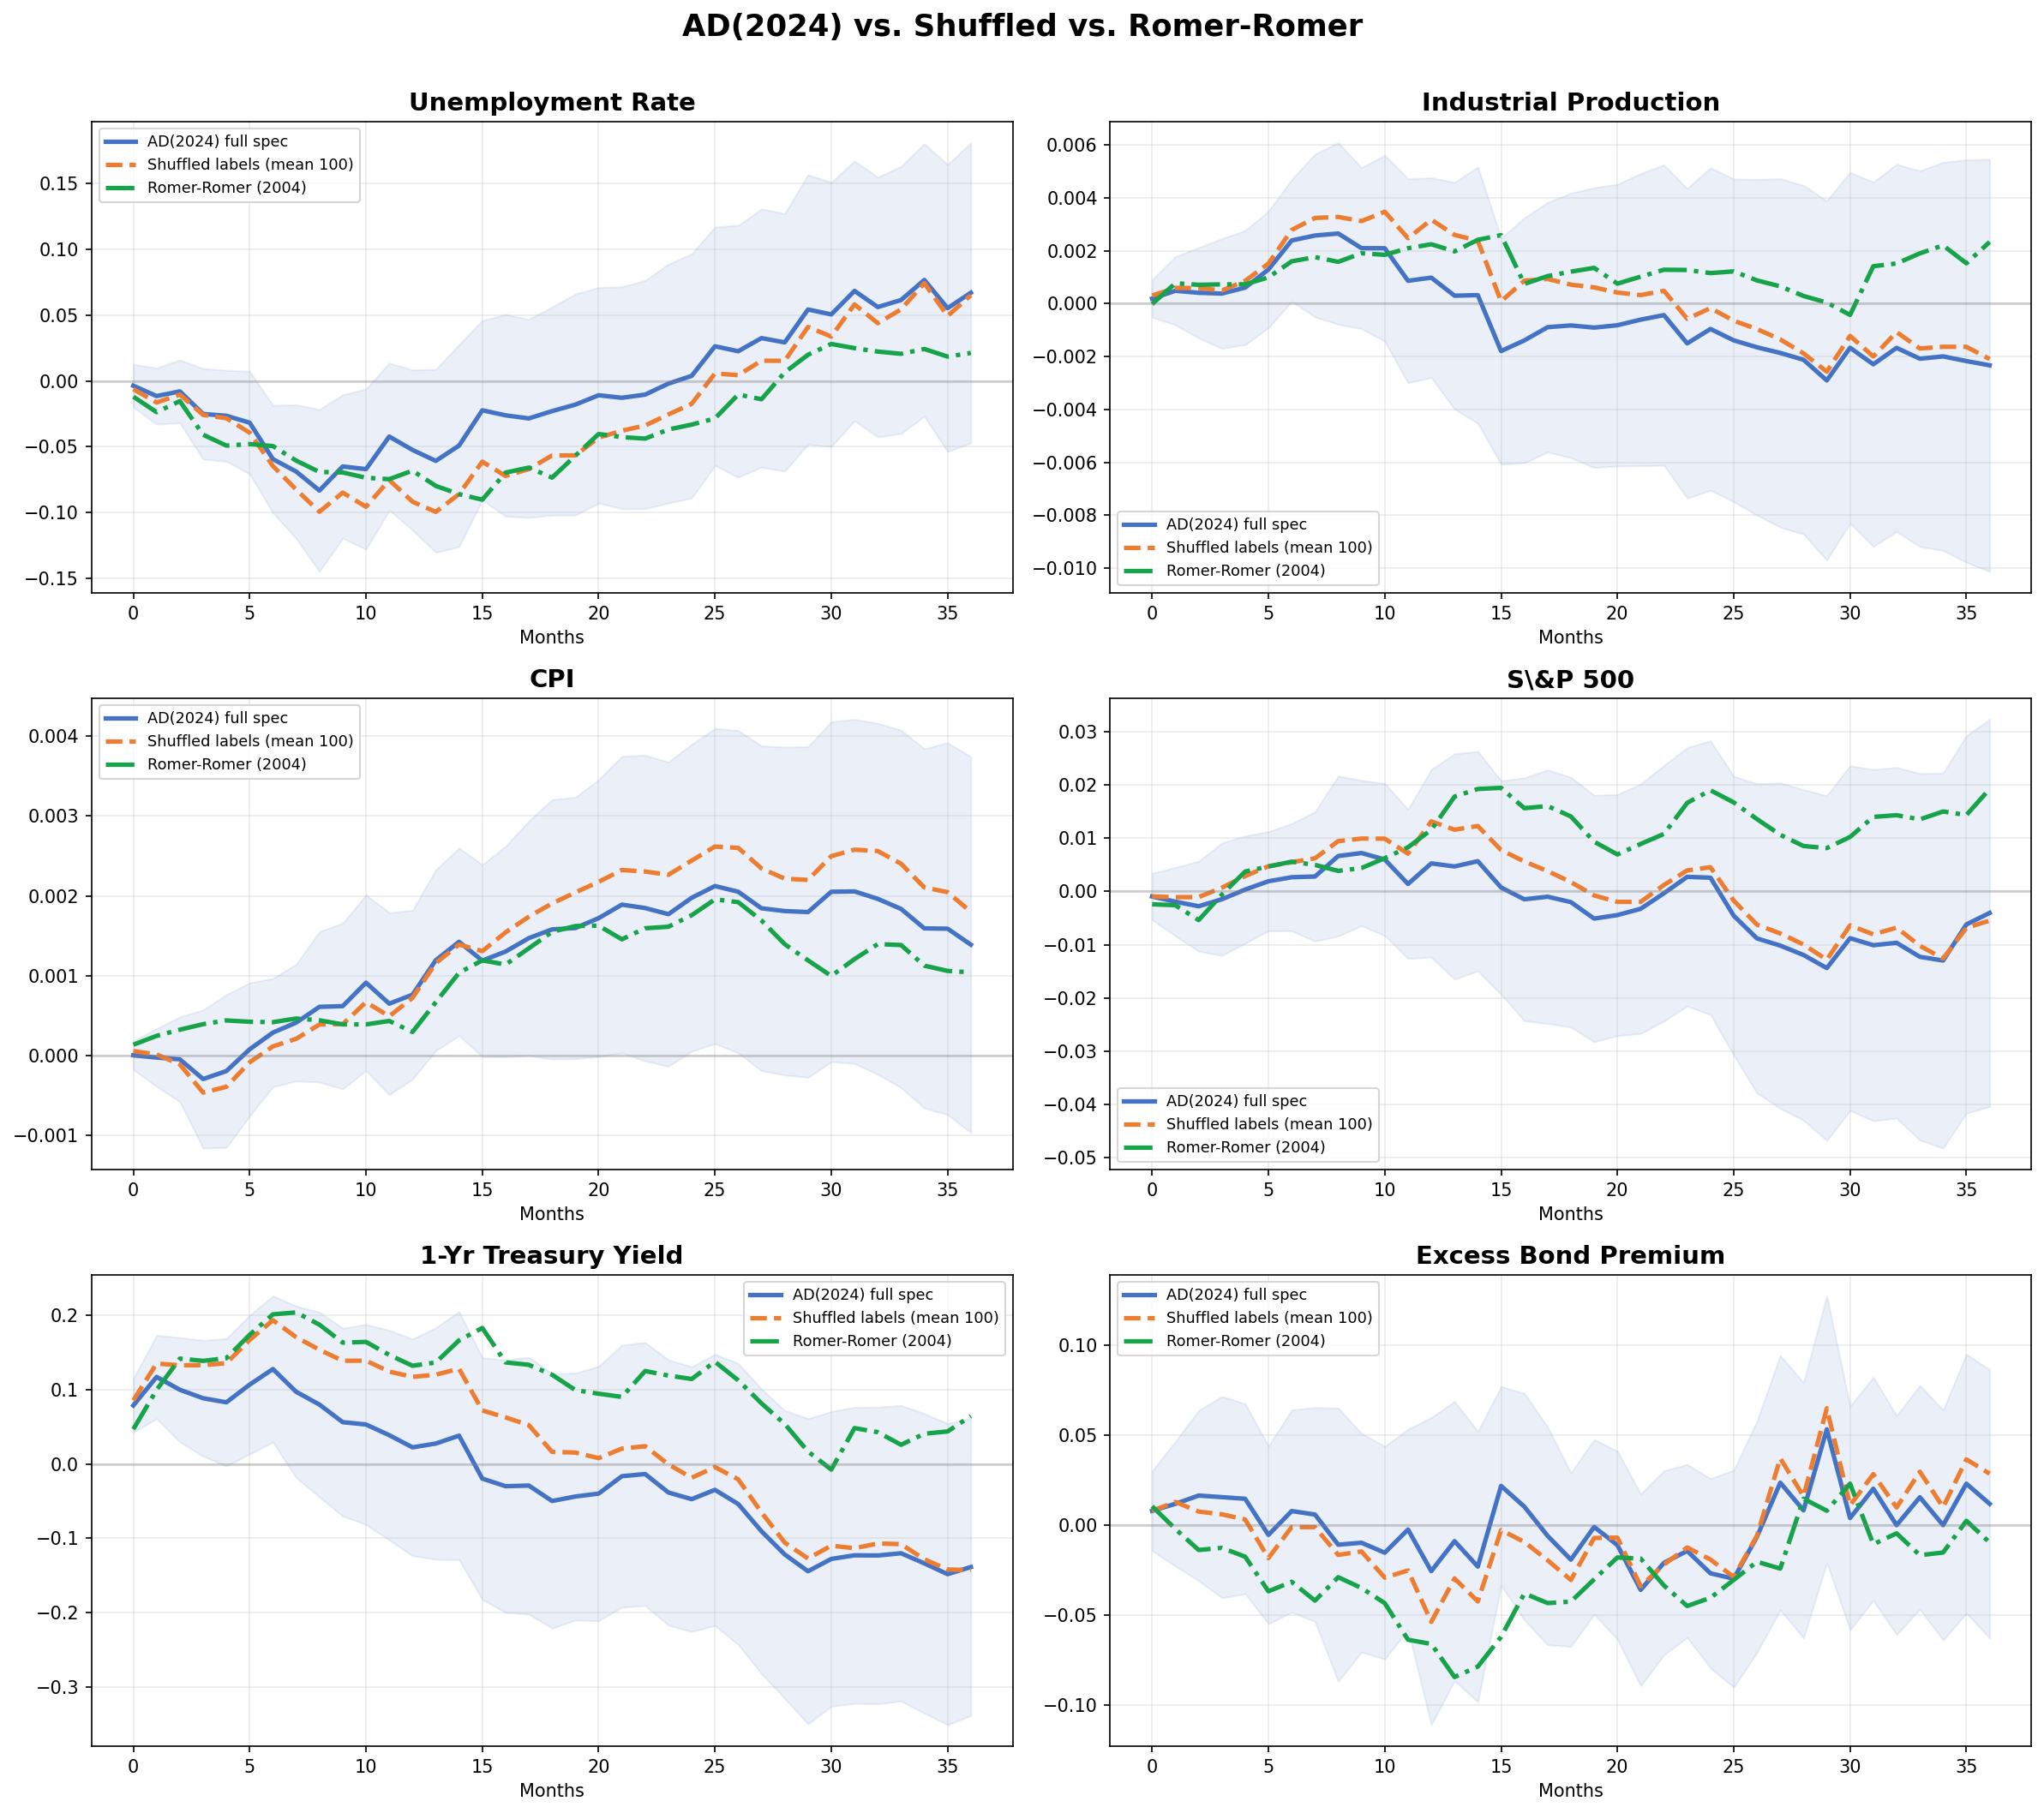
\includegraphics[width=0.92\textwidth]{../results/figures/irf_clean_comparison_v2.png}
\caption{Cumulative IRF to a 1-s.d.\ contractionary monetary shock. All series start at zero ($h=-1$, pre-shock). Shaded bands: 95\% Newey-West CI for the AD(2024) shock.}
\label{fig:irf}
\end{figure}

\textbf{AD(2024) and shuffled shocks produce essentially identical IRFs} across all six variables. The Romer-Romer shock yields noisier IRFs, consistent with its lower $R^2$ leaving systematic policy in the residual.

\textbf{Note on the CPI response:} The CPI IRF is positive following a contractionary shock, which is the canonical ``price puzzle.'' This may reflect the difference between LP and the BVAR framework used in AD(2024)'s Figure 6, or the absence of commodity price controls in our specification. We flag this for further investigation rather than claiming theory-consistency for the CPI panel.

% ======================================================================
\section*{7. Overfitting Diagnostics}
% ======================================================================

With $p/n = 15.8$, is the model overfitting?

\begin{table}[H]
\centering
\caption{Overfitting Diagnostics}
\label{tab:diag}
\begin{tabular}{lp{2.8cm}cp{2.2cm}}
\toprule
\textbf{Test} & \textbf{Method} & \textbf{Key Result} & \textbf{Conclusion} \\
\midrule
A. Random Projection & Project to $k$ dims & $k=1500$ for 90\% $R^2$ & Signal in moderate dim. \\
B. Bootstrap & 100 resamples & 5\% cross zero & Coefficients stable \\
C. Noise Injection & Add random noise & +10\%: $\Delta R^2 = +0.002$ & Reg. prevents overfit \\
D. Random Drop & Drop 50\% sentiment & $\Delta R^2 = +0.075$ & Note: increase suggests redundancy \\
E. Residual AC & Ljung-Box, DW & DW = 1.84 & Residuals white noise \\
\bottomrule
\end{tabular}
\end{table}

\textbf{Note on Test D:} In a correctly specified model, removing informative variables should \textit{reduce} $R^2$. The observed \textit{increase} of 0.075 when 50\% of sentiment variables are dropped suggests these variables are partially redundant rather than all independently informative---consistent with our finding that concept labels are incidental but dimensionality matters.

% ======================================================================
\section*{8. Summary}
% ======================================================================

\begin{enumerate}
    \item \textbf{Single-permutation shocks are nearly identical to the original} ($r = 0.947 \pm 0.005$). The mean-of-100 was not manufacturing the result. CV-selected $\lambda^*$ varies across permutations, but the shocks are robust to this variation.

    \item \textbf{Document tone (PC1) alone contributes almost nothing} ($\Delta R^2 = +0.014$). The 296 individual concepts contribute enormously ($\Delta R^2 = +0.455$), but this contribution is insensitive to label identity (shuffle drop $= 0.03$).

    \item \textbf{The value is in dimensionality, not labels.} 296 concepts $\times$ 5 lags create 1,480 time-varying sampling points. The specific concept names are incidental; the \textit{number} of sampling points is what enables Ridge to capture the document's temporal evolution.

    \item \textbf{AD(2024) shocks produce cleaner IRFs than Romer-Romer shocks,} confirming that text contains systematic policy information beyond numerical forecasts. Shuffled-label IRFs are essentially identical to the original.

    \item \textbf{The model does not overfit} despite $p/n = 15.8$. Ridge with $\lambda = 924$ successfully shrinks high-dimensional noise.
\end{enumerate}

\vspace{12pt}
{\small\color{gray} Code: \texttt{src/}. Results: \texttt{results/}. Presentation: \texttt{results/beamer\_presentation.pdf}.}

\end{document}
